\documentclass[class=minimal,border=0pt]{standalone}
\usepackage{tikz,amsmath, amssymb,bm,color}

\usetikzlibrary{shapes,arrows}
\usetikzlibrary{fit,backgrounds,positioning,calc}
\begin{document}
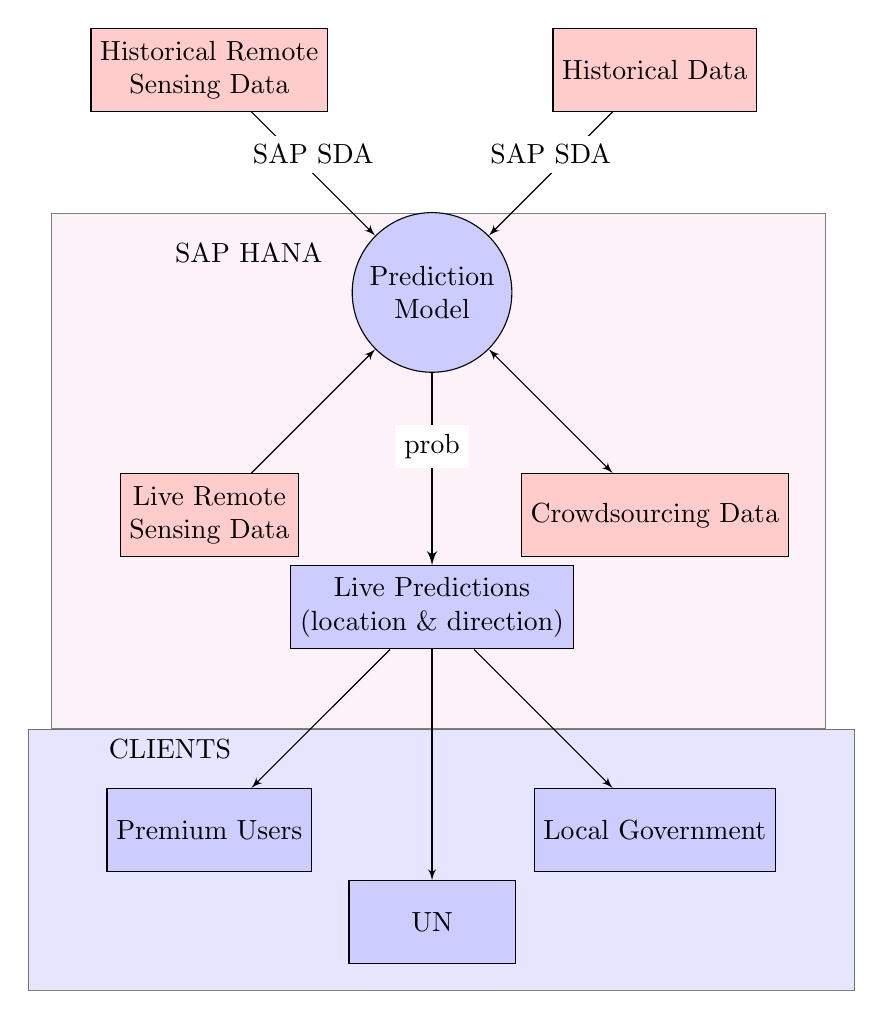
\begin{tikzpicture}[auto, align=center, node distance=4cm, >=latex']

%local definitions
\tikzstyle{DataSource} = [draw, fill=red!20, rectangle,minimum height=3em, minimum width=6em]
\tikzstyle{Client} = [draw, fill=blue!20, rectangle,minimum height=3em, minimum width=6em]
\tikzstyle{Product} = [draw, fill=blue!20, circle]
\tikzstyle{pinstyle} = [pin edge={to-,thin,black}]

\pgfdeclarelayer{background}
\pgfdeclarelayer{foreground}

%board components
	\node [Product] (PredictionModel) {Prediction\\Model};
	\node [DataSource, above left of=PredictionModel] (exData) {Historical Remote\\Sensing Data};
	\node [DataSource, above right of=PredictionModel] (exHistData) {Historical Data};
	\node [DataSource, below left of=PredictionModel] (lifeData) {Live Remote\\Sensing Data};	
	\node [DataSource, below right of=PredictionModel] (CrowdsourcingData) {Crowdsourcing Data};

	
	\node [Client, below of=PredictionModel] (lifePrediction) {Live Predictions\\(location \& direction)};

	\node [Client, below of=lifePrediction] (clientUN) {UN};
	\node [Client, below right of=lifePrediction] (clientGov) {Local Government};
	\node [Client, below left of=lifePrediction] (clientPU) {Premium Users};
	
	
%connections

	\draw [->] (exData) -- node[above,midway,fill=white]{SAP SDA} (PredictionModel);
	\draw [->] (exHistData) -- node[above, midway,fill=white]{SAP SDA} (PredictionModel);
	\draw [->] (lifeData) -- (PredictionModel);
	\draw [<->] (CrowdsourcingData) -- (PredictionModel);
	
	\draw [thick,->] (PredictionModel) -- node[above,midway,fill=white]{prob} (lifePrediction);

	%user connection
	\draw [->] (lifePrediction) -- (clientUN);
	\draw [->] (lifePrediction) -- (clientGov);
	\draw [->] (lifePrediction) -- (clientPU);


	%block names
	\node  at ($(PredictionModel -| exData)+(0.5,0.5)$) {SAP HANA};	
	\node (ClientStart)  at ($(clientPU.north)+(-0.5,0.5)$) {CLIENTS};	
	
\begin{scope}[on background layer]
	\filldraw [draw=black,fill=magenta!10,opacity=0.5] ($(PredictionModel -| exData)-(2,-1)$) rectangle ($(lifePrediction.south)+(5,-1)$);
	\filldraw [draw=black,fill=blue!20,opacity=0.5] ($(ClientStart.north)-(1.8,0)$) rectangle ($(clientGov.south east)+(1,-1.5)$);
	
\end{scope}




\end{tikzpicture}
\end{document}
